\documentclass{article}
	\usepackage[UTF8]{ctex}
	\usepackage{amsmath}
	\usepackage{graphicx}
	\usepackage{underscore}
	\usepackage{geometry}
	\usepackage{anysize}
	\usepackage{caption}
	\date{}
	\title{奋斗折线题解}
	\geometry{top=10mm,bottom=15mm,left=25mm,right=25mm}
	
	\begin{document}
		\maketitle \vspace{-50pt}
		
		\section{前提}
			\indent 本题求的是奋斗折线中最多的点的数目(后面统一称为求最长奋斗折线，最长奋斗折线的值为点的数目，而非折线的数量)。其中要求点的数目为偶数。我们可以把这个限制条件去掉，在求出最长奋斗折线后(从这里开始提及的最长奋斗折线都没有“点的数目为偶数”这个限制条件)，给出小于等于最大值的最大偶数即可。\\
			
			\indent 奋斗折线中，随着点的编号的递增，横坐标的坐标逐渐增大。按照横坐标对点进行排序，点的新编号为$1,2,\dots,n$。点s(缩写，指编号为s的点)扩展以点$1,2,\dots,t$作为终点的奋斗折线(需满足纵坐标的条件)，从而当前奋斗折线终点为点t，奋斗折线长度加1。其中t为横坐标与点s横坐标相同的点的最小编号减1。\\
			
		\section{贪心1}		
			若从一个点出发拓展奋斗折线(后一部分)得到最长奋斗曲线，那么以该点作为终点的奋斗折线(前一部分)选择以该点作为终点的奋斗折线中的最长奋斗折线。\\
			
			\indent 证明：\\
			
			\indent 反证法。\\
			
			\indent 一条奋斗折线有两个参数，最后一个点的纵坐标和折线的长度。其它条件都不会影响奋斗折线的拓展和折线的长度。\\
			
			\indent 设该点编号为d。设以该点作为终点的最长奋斗折线的长度为u，折线中的点编号依次为$a_{1},a_{2},\dots,a_{x-1},d,a_{x+1},\dots,a_{u}$。设当下选择的奋斗折线的长度为v($u\>v$)，折线中的点编号依次为$b_{1},b_{2},\dots,b_{y-1},d,b_{y+1},\dots,b_{v}$。\\
			
			\indent 若x,y同奇偶，则用$a_{1},a_{2},\dots,a_{x-1}$替代$b_{1},b_{2},\dots,b_{y-1}$，折线改为$a_{1},a_{2},\dots,a_{x-1},d,b_{y+1},\dots,b_{v}$，其长度更长，见图1-1、图1-2。\\
			
			\indent 若x,y不同奇偶，用$a_{1},a_{2},\dots,a_{x-1}$替代$b_{1},b_{2},\dots,b_{y-1},d$，折线改为$a_{1},a_{2},\dots,a_{x-1},b_{y+1},\dots,b_{v}$，其长度相同或更长，见图2-1、图2-2和图3-1、图3-2。
				\\\\
				
\begin{figure}
\begin{minipage}[t]{0.5\linewidth}
\centering
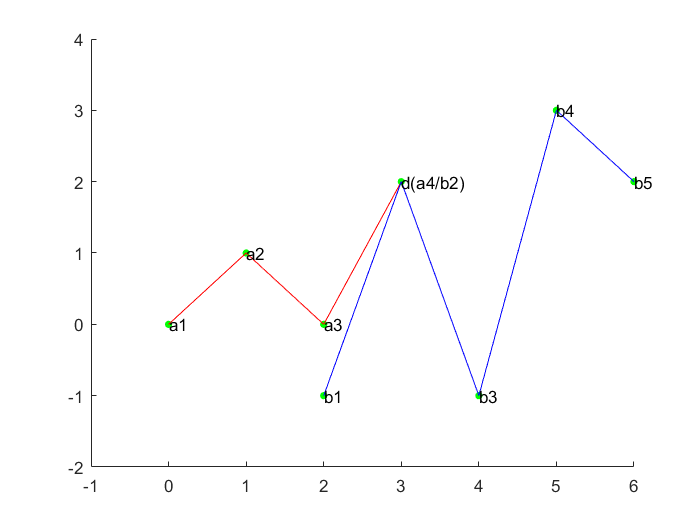
\includegraphics[width=3in]{1-1.png}
\caption*{图1-1}
\end{minipage}%
\begin{minipage}[t]{0.5\linewidth}
\centering
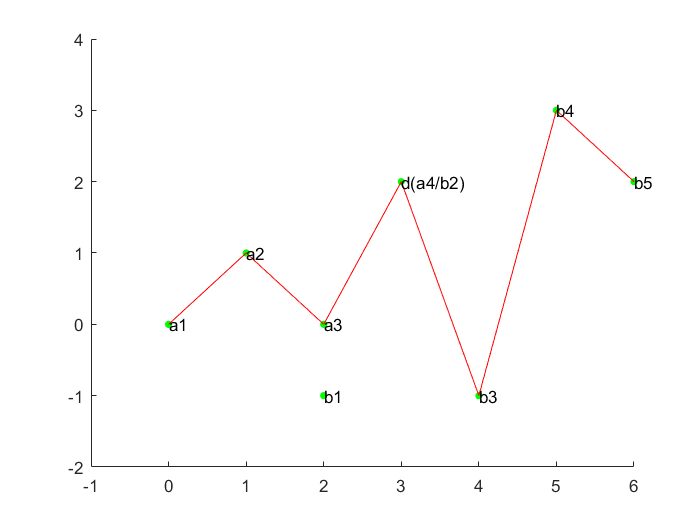
\includegraphics[width=3in]{1-2.png}
\caption*{图1-2}
\end{minipage}

\begin{minipage}[t]{0.5\linewidth}
\centering
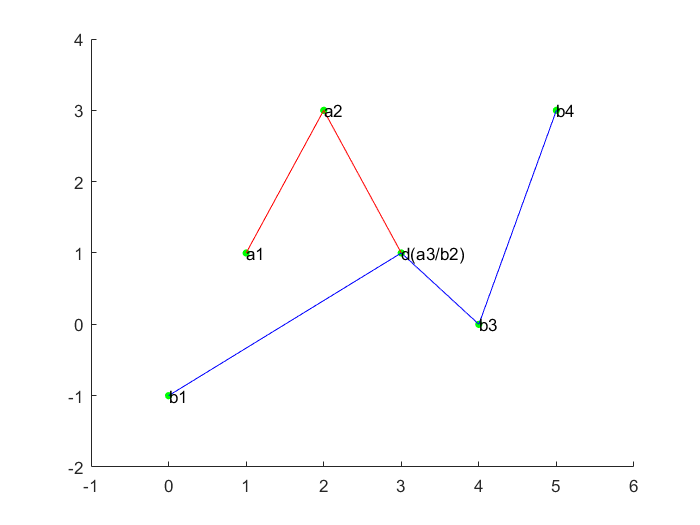
\includegraphics[width=3in]{2-1.png}
\caption*{图2-1}
\end{minipage}%
\begin{minipage}[t]{0.5\linewidth}
\centering
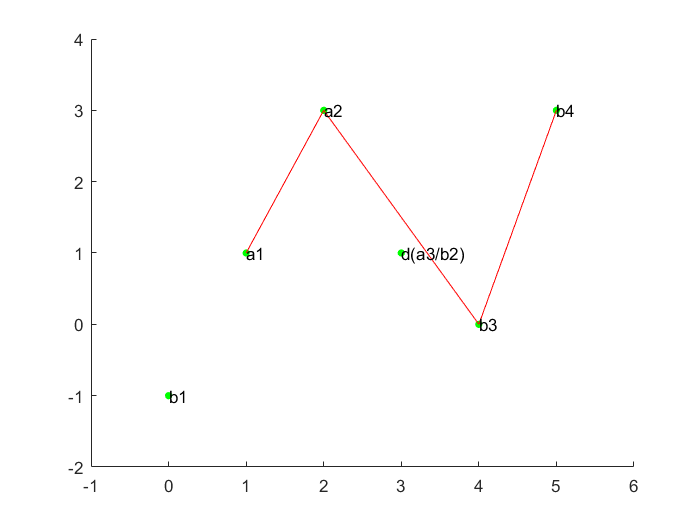
\includegraphics[width=3in]{2-2.png}
\caption*{图2-2}
\end{minipage}

\begin{minipage}[t]{0.5\linewidth}
\centering
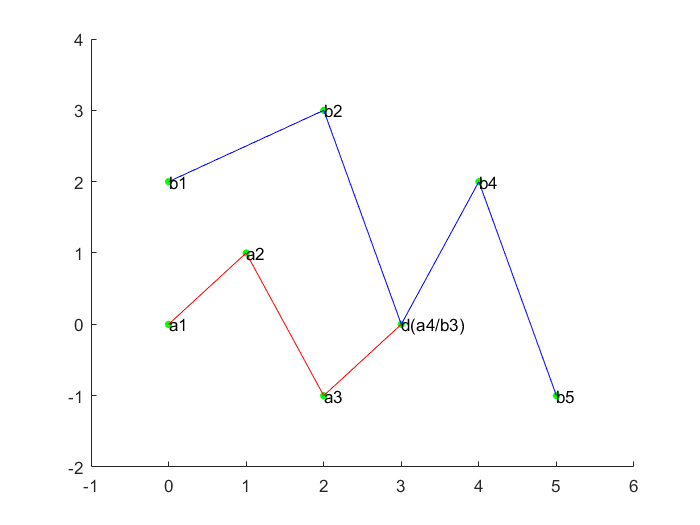
\includegraphics[width=3in]{3-1.png}
\caption*{图3-1}
\end{minipage}%
\begin{minipage}[t]{0.5\linewidth}
\centering
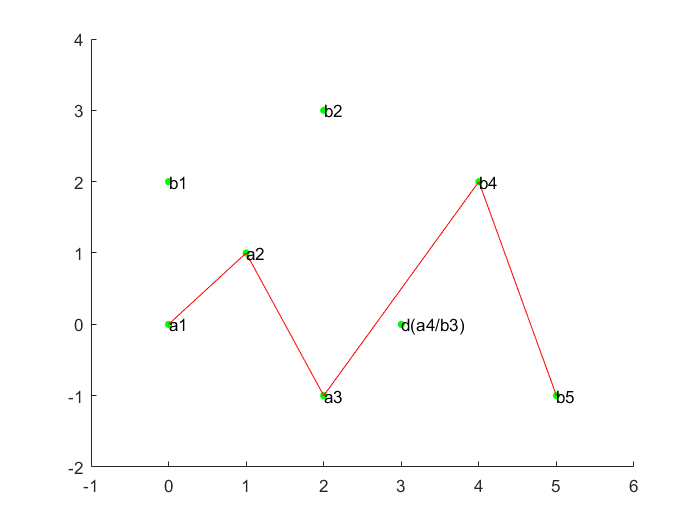
\includegraphics[width=3in]{3-2.png}
\caption*{图3-2}
\end{minipage}
\end{figure}
	
		\section{方法1：使用贪心1 \quad (排序+)dp}
		\indent 对点的横坐标进行排序。\\
		
		\indent 对于每个点，求出以该点作为终点的最长奋斗折线长度。以点s作为终点的奋斗折线是在终点为$1,2,\dots,t$其中一点的奋斗折线的基础上加上该点(需满足横坐标和纵坐标条件，见上文)。\\
		
		\indent 时间复杂度：O($n^{2}$)
		
		\section{贪心2}
		\indent 对所有横坐标相同的点进行合并，合并后点的编号为$1,2,\dots,n'$，每个点都有纵坐标下界和上界，当该点在奋斗折线出现时，纵坐标选择纵坐标下界和上界之间的一个值(同横坐标的点最多只能选择一个)。\\
		
		\indent 按照编号从小到大的顺序加入点，满足横坐标从小到大的要求。按照其它的顺序加入点(奋斗折线在之前的某一点i作为奋斗折线的终点的基础上加入了一个新的点j($i>j$))，都不满足横坐标的要求。\\
		
		\indent 设最佳奋斗折线是长度最长的奋斗折线，当有多条奋斗折线长度相同时，选择终点的纵坐标最大(长度为偶数)/纵坐标最小(长度为奇数)的奋斗折线。\\
		
		\indent 求得使用前s($s \in [1,n']$)个点的最佳奋斗曲线，也就是求得了使用前s($s \in [1,n']$)个点的最长奋斗曲线(其中一条)。\\
		
		\indent 前s($s \in (1,n']$)个点的最佳奋斗曲线是通过前s-1($s \in (1,n']$)个点的最佳奋斗曲线得到的。\\

		\indent 方法为：\\
		
		\indent 如果新点可以加入到前s-1($s \in (1,n']$)个点的最佳奋斗曲线中(如果前s-1($s \in (1,n']$)个点的最佳奋斗曲线的长度为奇数，采用纵坐标上界，否则采用纵坐标下界)，则加入；否则新点替代原有前s-1($s \in (1,n']$)个点的最佳奋斗曲线的终点。\\
		
		\indent 更详细的来说：\\
		
		\indent \textcircled{1} 若前s-1($s \in (1,n']$)个点的最佳奋斗折线需要上升(当前长度为奇数)，若新点(纵坐标采用上界)比原折线终点的纵坐标大，则折线终点改为新点(纵坐标采用上界)，折线长度加1，否则新点最小的纵坐标必小于等于原折线终点，折线终点改为新点最小的纵坐标，折线长度不变。\\
		
		\indent \textcircled{2} 若前s-1($s \in (1,n']$)个点的最佳奋斗折线需要下降(当前长度为偶数)，若新点(纵坐标采用下界)比原折线终点的纵坐标小，则折线终点改为新点(纵坐标采用下界)，折线长度加1，否则新点(纵坐标采用上界)的纵坐标必大于等于原折线终点，折线终点改为新点最大的纵坐标，折线长度不变。\\
		
		\indent 更简单的来说：\\
		
		\indent 对于一个新的点，如果可以延伸则延伸，否则改善(至少不变)。\\
		
		\indent 证明：\\
		
		\indent \textcircled{1}使用之前的最佳奋斗折线延伸，这个方法(对于一个新的点，如果可以延伸则延伸，否则改善(至少不变))，在使用之前的最佳奋斗折线进行延伸得到的所有奋斗折线中是最佳奋斗折线。\\
		
		\indent 根据定义，易得证。\\
		
		\indent \textcircled{2}使用非最佳奋斗折线进行拓展，与使用最佳奋斗折线相比，肯定做不到比最佳奋斗曲线好。\\
		
		\indent 证明方法与贪心1的证明方法很类似。\\
		
		\indent 若非最佳奋斗折线与最佳奋斗折线的长度同奇偶(只考虑一致，其它易证)，那么对于最后一个点，最佳奋斗折线的点的纵坐标比非最佳奋斗折线的点的纵坐标“好”，因为对于后续点，存在最佳奋斗折线的钟点可以延伸，非最佳奋斗折线的钟点不可以延伸的情况；而当非最佳奋斗折线的种点可以延伸时，最佳奋斗折线的钟点必定可以延伸。\\
		
		\indent 若非最佳奋斗折线与最佳奋斗折线的长度不同奇偶(只考虑相差1，其它易证)，那么非最佳奋斗折线不加上这个点必定比最佳奋斗折线差，若加上这个点，其长度也只能与之前的最佳奋斗折线的长度一致。而之前的最佳奋斗折线加上该点，要么长度加1，要么最后一个点改为该点，即不会比使用任意非最佳奋斗折线进行扩展差。

		\section{方法2：使用贪心1+贪心2 \quad 排序+贪心}
		
		\indent 对点的横坐标进行排序。所有横坐标，记录上界和下界的值。\\
		
		\indent 最佳奋斗曲线的修改见上文。\\
		
		\indent 时间复杂度：O($nlogn$)
		
		\section{总结}
		贪心不难想到，但证明很难。这时候，直接写就好了！(有一种东西叫直觉)\\
		
		多个点的横坐标相同的情况及处理方法比较易忽略，是本题的其中一个重要考点。
	\end
	{document}